\section{idées}
\begin{itemize}
\item spatial/temporel sophie lebre loic aussi sur les ruptures
\item EM/VEMtree/PLN étude simul des modèles qui se basent sur PLN
\item couche observée vraisemblance composite
\item la sélection de modèles
\item comparaison de réseau : des calculs qu'on sait faire entre des matrices de proba (proba qu'une arête soit commune à deux réseaux ) etc.
\end{itemize} 

\section{Network inference from PLN}

\begin{figure}
\centering
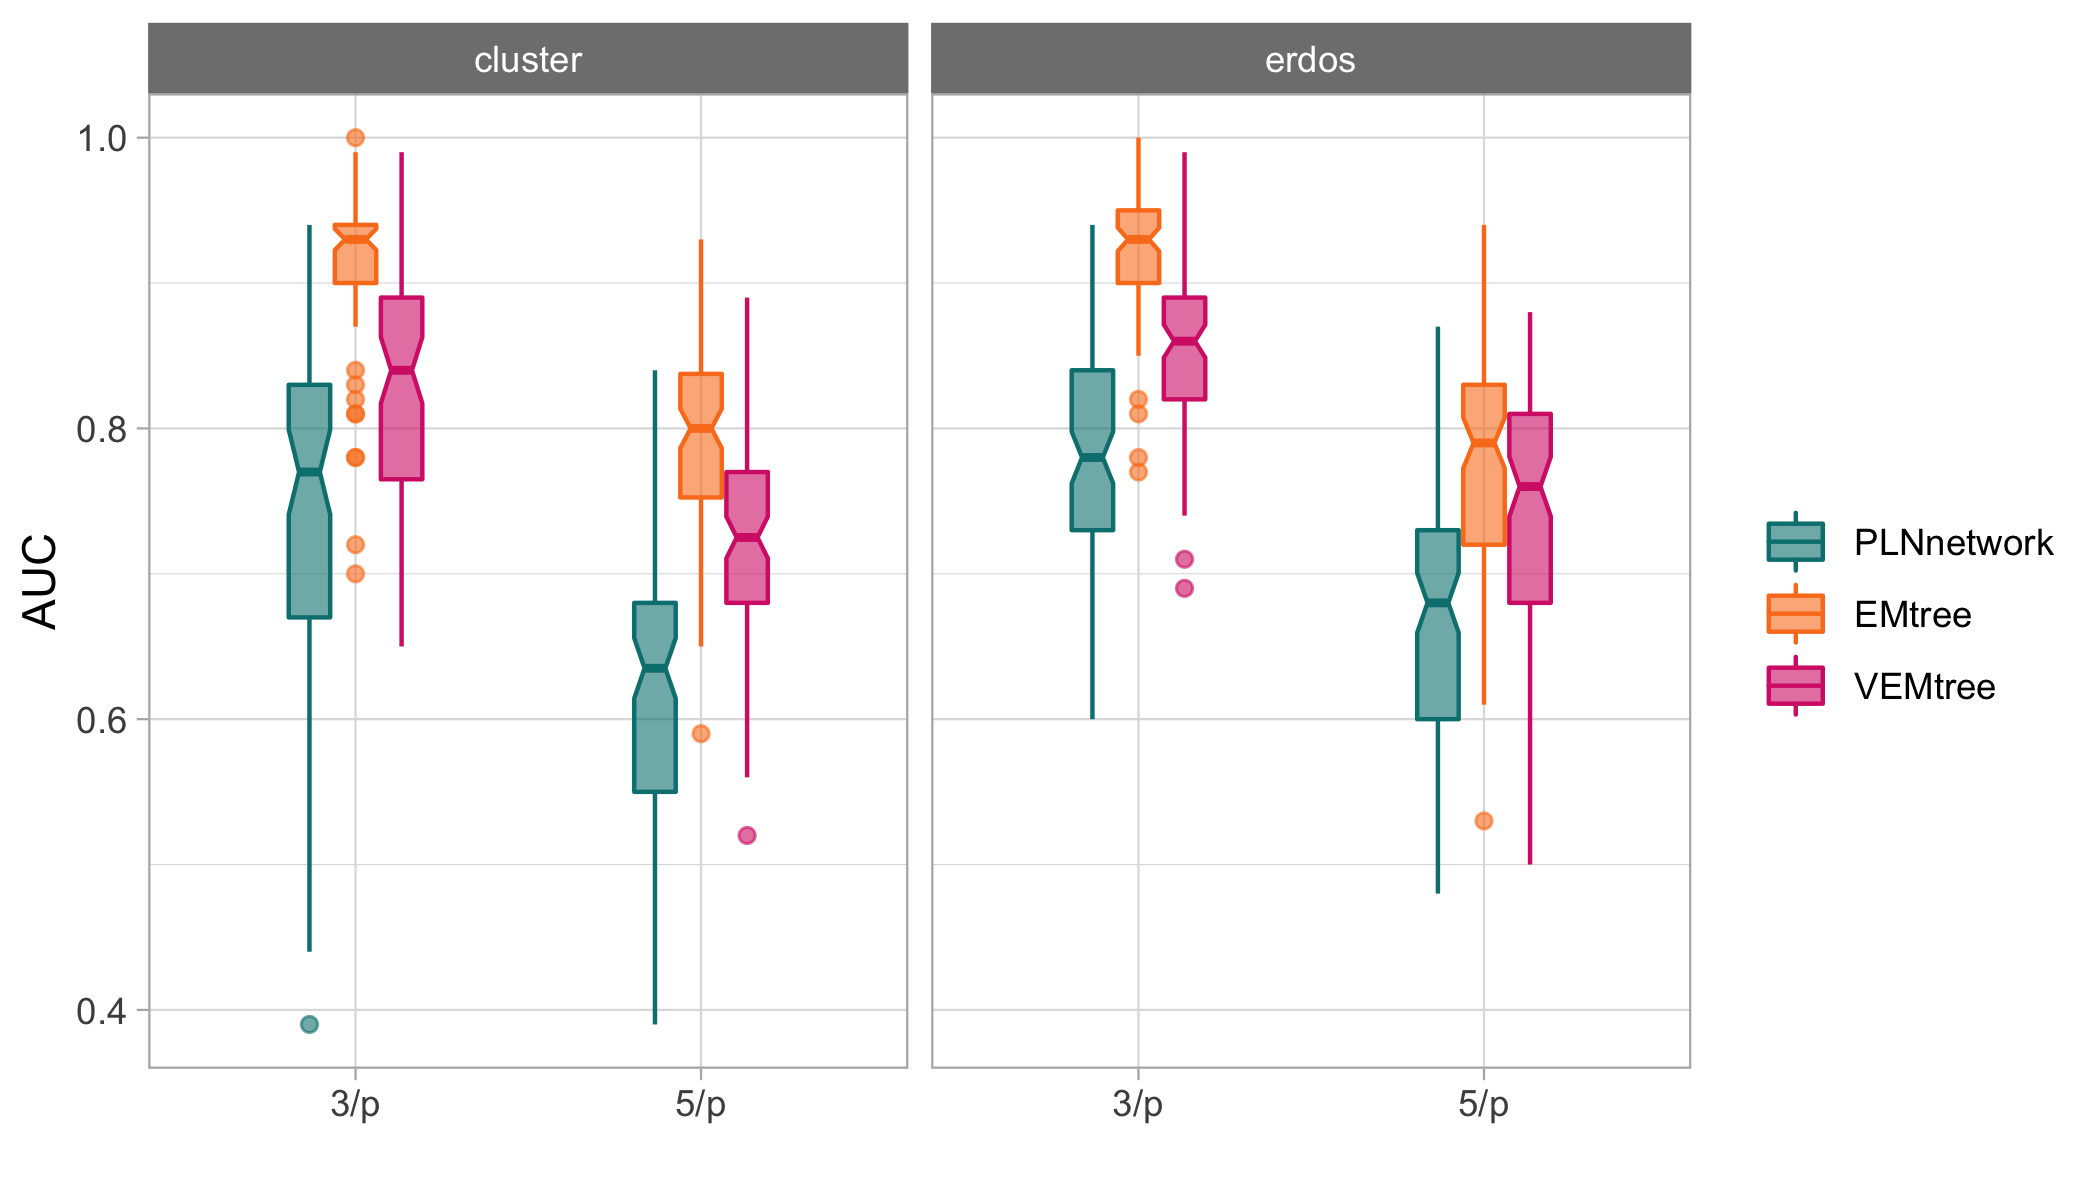
\includegraphics[width=12cm]{figs/AUC_PLN_EM_VEM.png}
\end{figure}
\begin{figure}
\centering
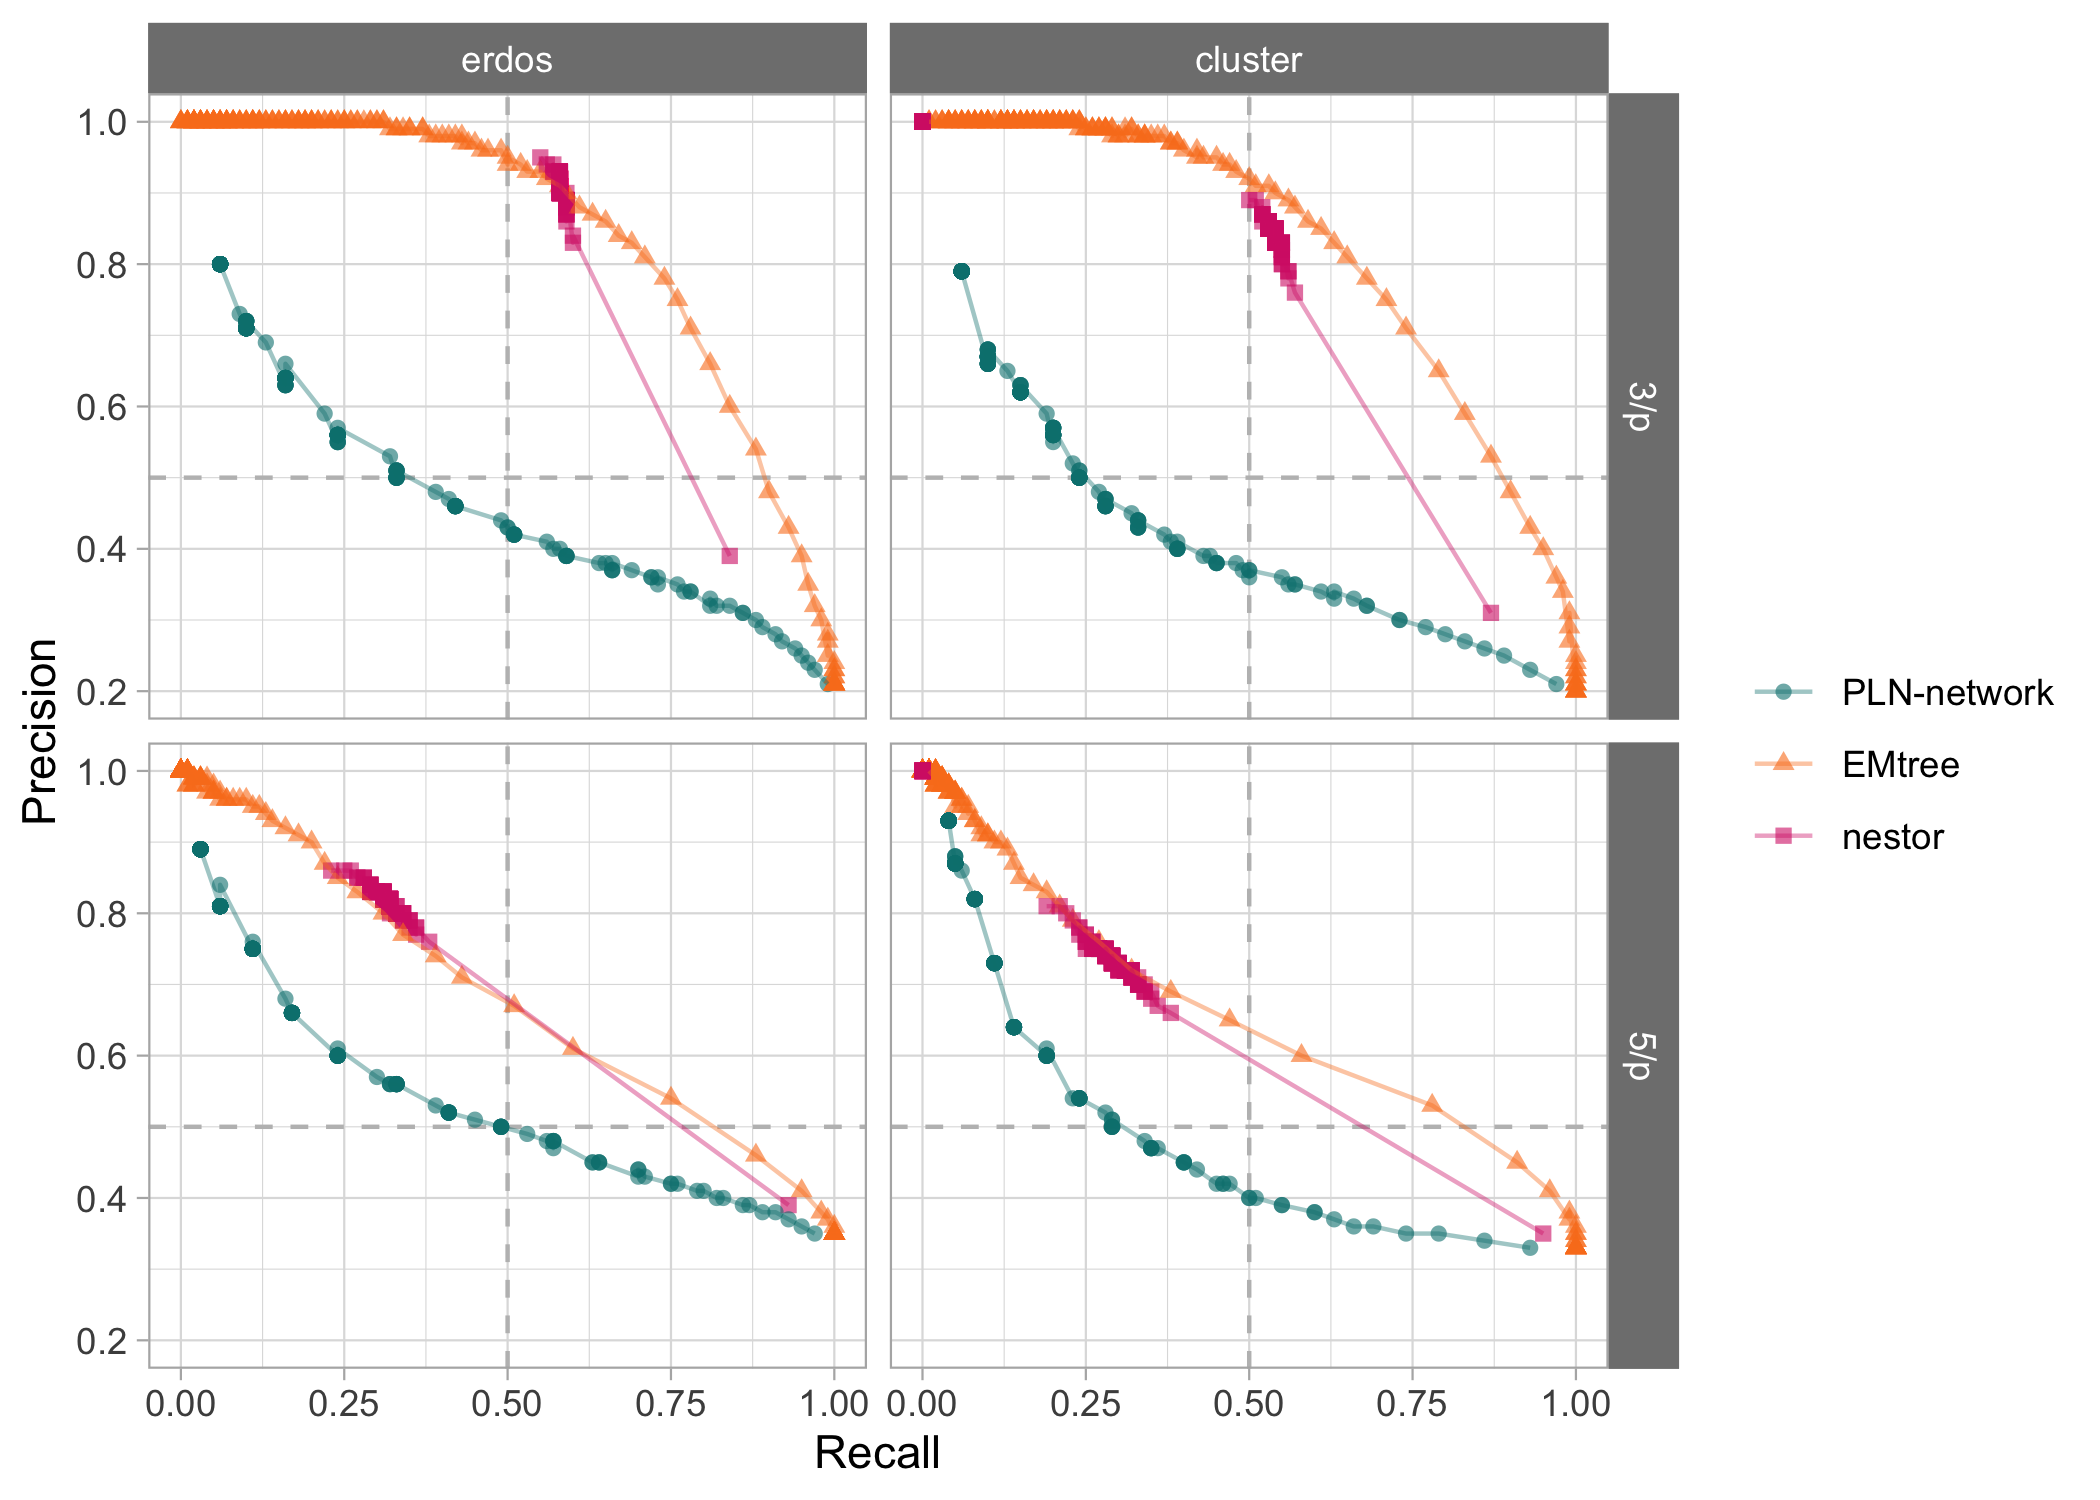
\includegraphics[width=12cm]{figs/precrec_PLN_EM_VEM.png}
\end{figure}

with $min.ratio=1\cdot 10^{-3}$ for PLNnetwork